\documentclass[a4paper, 11pt, twocolumn]{article}
\usepackage{caption}
\usepackage{graphicx}
\usepackage{color} %colors in text
\usepackage{textcomp} % mai multe:-??
\usepackage[T1]{pbsi} %hand writting nice :P
\usepackage[T1]{fontenc} %mai multe fonturi
\usepackage{mathrsfs} % letters for math
\usepackage{fullpage} % fara margini
\usepackage{amsmath} % formule matematice
\usepackage[all]{xy} % pt desenat
\usepackage{listings}
\usepackage{algorithmic}
\usepackage{algorithm}
\usepackage{amssymb}
\usepackage[parfill]{parskip}
%\usepackage{palatino, url, multicol} %multicolumns
\definecolor{gray}{rgb}{0.7,0.7,0.7} 
\usepackage{enumerate} %for enumerate
\fontfamily{ccbr}\selectfont\normalsize
\newcommand{\ds}{\displaystyle}
\newcommand{\todo}[1]{\textcolor{red}{\textbf{#1}}}
\newcommand{\fade}[1]{\textcolor{gray}{\textbf{#1}}}
%\hyphenpenalty=100000
\date{} % fara data
\author{\fade{Nimrod Raiman [0336696]}\\\fade{Silvia L. Pintea [6109960]}}
\title{Rock, Paper \& Scissors with Nao}
\begin{document}
    \maketitle
	%ABSTRACT SECTION__________________________________________
    \abstract{Throughout this paper we are going to try to explain our work on teaching a humanoid robot (\emph{Nao}) to play \emph{"Rock, paper \& scissors"}. In order to accomplish this task we have used different theoretical methods which are described in the section~\ref{sec:methods}. The next section presents our experimental results. Finally we give an overall view of this paper and indicate the possible further work that could be done on this subject.}  
	%SECTION SECTION_________________________________________
    \section{Introduction}
	\label{sec:intro}
        \emph{"Rock, Paper \& Scissors"} is an easy and well known game. This is the reason for which it is interesting to learn a robot how to play it against human players. In order to do that the robot needs to be able to recognize the hands of its opponent and classify the gesture as: \emph{"rock"}, \emph{"paper"} or \emph{"scissors"}.\\	
		\hspace*{10px}In this paper we describe our approach to accomplish this in real time. Our solution is fairly robust to lightning condition and also the gestures of the player need not be restricted to certain angles or positions in the frame.\\ 
        \hspace*{10px}Our problem has been split into three main tasks: extracting the hands from the webcam stream, recognizing the gesture of the extracted hand and implementing motion and speech on \emph{Nao}. Throughout our project we have tried different approaches in order to find the best method to solve the problem.\\
		 \hspace*{10px}We have experimented with methods such as: \emph{backprojection} of pixels values for hand detection, \emph{Gabor filters} and \emph{PCA} for classifying signs. We will start by describing the methods that we have tried to use and then continue by giving an overview of the results and the conclusions.   
	%METHODS SECTION__________________________________ 
    \section{Methods}
	\label{sec:methods}
		For hand detection and recognition we have tried two different techniques: a naive approach and the backproject of the pixels corresponding to skin.\\
		\hspace*{10px}For the gesture recognition we have experimented with different sets of data and we have extracted different features using methods such as: \emph{PCA}, \emph{Gabor filters}. We have also tried using two different types of classifiers: \emph{SVM} (support vector machine) and \emph{Knn} (K nearest neighbors).\\
		\hspace*{10px}We will continue by giving a more detailed description of the methods employed. 
        \subsection{Hands extraction}
		\label{sec:Meth_exrctHands}
        \subsubsection{Naive approach}
		\todo{Nimrod .....}\\

        \subsubsection{Backprojection of skin pixels}
        \todo{Nimrod .....}\\
        Determine hue and saturation values for skin color\\
        Threshold the image with hue and saturation values\\
        Use erosion \& dilation\\
        Find ares corresponding to hands\\
        vspace*{10px}
        Robust/sophisticated approach\\
        Determine skin color histogram\\
        - Detect face\\
        - Build histogram of pixels corresponding to the face\\
        Backproject skin color histogram on whole frame\\
        Use erosion \& dilation to reduce the noise and fill up gaps\\
        Extract area of corresponding to the hand\\
        Use more sophisticated erosion \& dilation on hand area\\
        - Retain the hand and remove the background\\
        - Resize the area of interest to 70x70

        \subsection{Gesture recognition}
		For the gesture recognition task we have started by using a training set containing images of hands of \emph{70$\times$70}px with different backgrounds. The problem proved to be too complex for our classifiers so we have decided to switch to a simpler one which would contain only centered hands and a black background.\\ 
		\hspace*{10px}Out of this dataset we have extracted the features to be using during the classification.
		\label{sec:Meth_clssifyHands}
		\subsubsection{PCA}
		\todo{Silvia .....}\\

		\subsubsection{Gabor filters}
		\begin{flushleft}
		\begin{figure}[!hbtp]
		   \centering
		   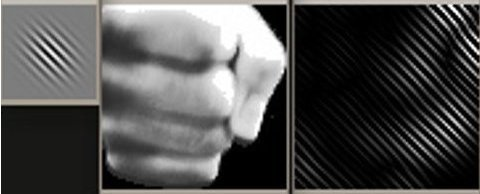
\includegraphics[width=0.45\textwidth]{gabor.jpg}
	   	\end{figure}	
		\end{flushleft}

		\todo{Sivlia .....}\\

		\subsubsection{Classification}
		\todo{Silvia .....}\\


        Do we want subsub sections here?\\\\
        Build reliable training set\\
        Find useful features to train on: PCA, Gabor wavelets, grayscale images\\
        Train a classifier: Knn /SVM\\
        Create models \& test in order to find the best one\\
        
        \subsection{Motion \& Speech on Nao}
		\label{sec:Meth_naoPlay}
        How does Nao play Rock!Paper!Scissors!\\\\
        Make Nao generate the moves for "rock", "paper" and "scissors"\\
        I Make Nao keep the score of the game by recognizing the gestures of the
        other player
	%EXPERIMENTAL RESULTS SECTION_______________________________________ 
    \section{Results}
	\label{sec:results}
    	Some nice results here...\\
		\begin{table}[!hbtp]
		\begin{tabular}{| c | c | c |}
			\hline\hline
			\textbf{Size} & \textbf{Method} & \textbf{Average Error}\\ 
			\hline\hline
			  70$\times$70 & \emph{PCA} & 0.475\\
			\hline
			  20$\times$20 & \emph{PCA} & 0.470\\
			\hline
			  20$\times$20 & \emph{Gabor} & 0.021\\
			\hline
			  20$\times$20 & \emph{Gabor + PCA} & 0.510\\
			\hline
			  \textbf{20$\times$20} & \textbf{\emph{Gabor \& Image}} & \textbf{0.012}\\
		 	\hline
			  20$\times$20 & \emph{(Gabor \& Image)} & 0.447\\
		               & \emph {+ PCA}  &     \\ 			
			\hline
			  70$\times$70 & \emph{Grayscale} & 0.016\\
			\hline
			  20$\times$20 & \emph{Grayscale} & 0.014\\
			\hline
		\end{tabular}
		\caption{Average errors for different methods}
		\end{table}

	%CONCLUSIONS & FARTHER WORK SECTION________________________________
    \section{Conclusions}
	\label{sec:conclusion}
    	Conclusion\\
   	 	What now?
    %BIBLIOGRAPHY SECTION______________________________________________
	\begin{thebibliography}{2}
		\bibitem{gwenns}
		Yen-Ting Chen, Kuo-Tsung Tsen, \emph{Developing a Multiple-angle Hand Gesture Recognition System for Human Machine Interaction}; 2007
		\bibitem{gabor}
		M. R. Tuner, \emph{Texture Discrimination by Gabor Functions}; 1986, Biol. Cybern. 55, p. 71-82 
	\end{thebibliography}    
\end{document}



